\documentclass[11pt,letterpaper,boxed]{pset}

\usepackage[margin=0.75in]{geometry}
\usepackage{ulem}

\name{Name: \rule{2.5cm}{0.15mm}}
\assignment{Box \# \rule{1.5cm}{0.15mm}}
\class{MATH065 HW9}
\duedate{04 June 2019}

\begin{document}

    \problemlist{MATH065 Homework 9}
    
    \afterpage{\blankpage}
    \begin{problem} [Exercise 1.]  
        An automobile suspension system can be modeled by a coupled mass-spring system where $m_1$ is the car body, $m_2$ the wheel/tire assembly, and the dashpot $c$ is a shock absorber:
        
         \begin{eqnarray}
             m_1 \, x''  & = &  -k_1 (x-y)  - c(\dot{x} - \dot{y}) \\
             m_2 \, y'' &  = &  - k_2 y  - k_1 (y-x) - c(\dot{y} - \dot{x})
         \end{eqnarray}
         
        Here $x$ and $y$ denote displacement from static equilibrium for mass $m_1$ and $m_2$, respectively (arrows indicate the positive direction), $k_1$ and $k_2$ are spring constants, and $c > 0$ is the damping coefficient.
        
        \[  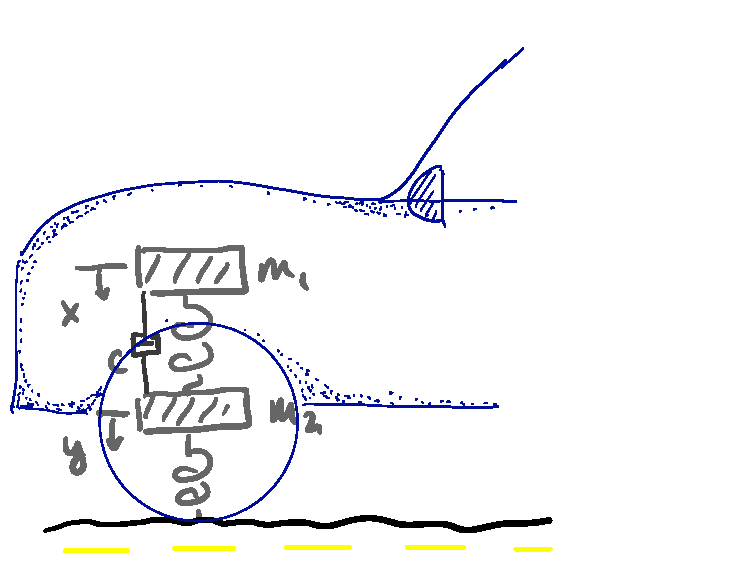
\includegraphics[width=0.35\textwidth]{suspension.pdf}  \]
        
        \begin{enumerate}
            \item[(a)]   Introduce state variables to rewrite the system of second order DEs (1)-(2) as a first order system  $\mathbf{x} ' = A \, \mathbf{x}$ and identify the matrix $A$. Each second order equation corresponds to  two first-order equations, so we are expecting a $4 \times 4$ matrix $A$. This is consistent with the system's four degrees of freedom (position/velocity for each mass). 
            \item[(b)] Assume $c = 0$ (no damping) and use a calculator or computer to determine the eigenvalues of your matrix $A$ when $m_1=m_2=1, k_1=3, k_2=2$. These eigenvalues define the ``natural frequencies" for the system with these parameters. We know the flow via $e^{At}$ will involve exponential functions with $e^{\lambda t}$ for these eigenvalues. Given this, do your eigenvalues seem appropriate for this undamped case?
            \item[(c)] Suppose we add damping, say $c=4$. What are the eigenvalues of $A$? What changed and does the change seem appropriate? 
        \end{enumerate}
        
        \textbf{Note}: The road introduces an external forcing that leads to the inhomogeneous system $\mathbf{x} ' = A \, \mathbf{x} + \mathbf{F}.$ One can study the car's response to various road conditions (e.g., wavy road modeled by a periodic function) and then try to design the system (adjusting physical properties to change any of the parameters $k_1, k_2, m_1, m_2, c$) in order to avoid resonance, where the system's natural frequencies match the external forcing (e.g., when you hit certain speeds and everything starts to rattle in the vehicle!). 
    \end{problem}
    \newpage
    
    
    \begin{problem} [Exercise 2.]
        The five points of this exercise are dedicated to the clarity, precision, and style of your write up to the next exercise.  This means first working out all the details before writing up your solution (bonus points for creative write ups!). 
    \end{problem}
    
    
    \begin{problem} [Exercise 3.] 
        Solve the initial value problem
        
        \begin{eqnarray*}
            \dot{x} &=& 2 y + \cos \omega t \\
            \dot{y} &= &  - 2 x + \sin \omega t
        \end{eqnarray*}
        
        where $x(0)=a, y(0) =b,$ and $\omega \neq 0$. Make sure your solution is valid for \textit{all} values of $\omega \neq 0$ (i.e., be careful not to divide by $0$; if a given step leads to division by $0$ then you have to go back one step and reconsider the calculation more specifically in that case).  
    \end{problem}
    \newpage
    
    \begin{problem} [Exercise 4.]
        Introduce state variables in order to write each of the following differential equations as an equivalent  first-order system $\mathbf{x}' = \mathbf{f}(\mathbf{x})$. Find all equilibrium points for your system. 
    
        \begin{enumerate} [(a)]
            \item (\textbf{van der Pol}) 
            
                \[\ddot{u} + \lambda  (u^2 - 1) \dot{u} + u = 0\] 
            
            where $\lambda > 0$. This is an important model in the theory of oscillations, famous enough to have its own wiki page (Balthasar van der Pol introduced the equation to model oscillatory electrical activity in the heart).
            \item (\textbf{Pendulum}) 
                
                \[  \ddot{\theta} + c \dot{\theta} + \lambda \sin \theta = 0 \]
                
            which models a damped pendulum where $\theta(t)$ is the angle from static equilibrium, $c > 0$ is a damping constant, and $\lambda = \sqrt{g/L}$ (gravity over length).
        \end{enumerate}
    \end{problem}
    \newpage
    
    
    \begin{problem} [Exercise 5.]
        Consider the SIR Model:
        
        \begin{eqnarray*}
            \dot{S} & = & -\alpha S I \\
            \dot{I} & = &  \alpha S I  - \beta I  \\
            \dot{R} & = & \beta I
        \end{eqnarray*}
        
        where $\alpha,\beta  > 0$ are constants (infection and recovery rate, respectively).   
        
        \begin{enumerate} [(a)]
            \item Show that the total population $N = S+I+R$ remains constant. Hint: What is $\dot{N}$?
            \item Given the total population remains constant we typically scale by $N$ so that the state variables lie between $0$ and $1$ and represent the fraction of the population that is susceptible, infected, or recovered. Assuming this is the case, find all equilibrium points of the system and explain what the equilibrium points physically corresponds to with respect to the population.
        \end{enumerate} 
    \end{problem}
    \newpage
    
    \begin{problem} [Exercise 6.]
        ({\bf The Lorenz Equations}) Consider the  nonlinear system
        
        \begin{eqnarray*}
            x' & = & \sigma ( y - x) \\
            y' & = & r x - y - x z \\
            z'  & = & -\beta z + x y
        \end{eqnarray*}
        
        where $\sigma,  r,$ and $\beta$ are positive constants. To simplify, let $\beta=1$ and $\sigma=3$. Show that for $0 < r < 1$ the system has only one equilibrium point while for $r>1$ the system has three equilibrium points. 
    \end{problem}
    \newpage

\end{document}